\documentclass[times, utf8, zavrsni]{fer}
\usepackage{booktabs}
\usepackage{pdflscape}
\usepackage{enumitem}
\usepackage{ulem}
\usepackage{listings}


\lstset{language=SQL,
    basicstyle=\ttfamily,
    frame=single,
    breaklines=true,
    showstringspaces=false,
    columns=flexible,
    belowskip=\baselineskip
}

\renewcommand{\baselinestretch}{1.5}

\begin{document}

% TODO: Navedite broj rada.
\thesisnumber{000}

% TODO: Navedite naslov rada.
\title{Baza podataka i web-aplikacija za plivačka natjecanja}

% TODO: Navedite vaše ime i prezime.
\author{Ilan Vezmarović}

\maketitle

% Ispis stranice s napomenom o umetanju izvornika rada. Uklonite naredbu \izvornik ako želite izbaciti tu stranicu.
% \izvornik

% Dodavanje zahvale ili prazne stranice. Ako ne želite dodati zahvalu, naredbu ostavite radi prazne stranice.
\zahvala{}

\tableofcontents

\chapter{Uvod}
U današnjem dobu digitalne revolucije, postoji sve veća potreba za praćenjem i analizom sportskih rezultata. 
Plivanje je jedan od sportova za koji je izražena potreba za pohranom velikog broja informacija.
Rezultat navedenog je velik broj sportskih aplikacija. Kod aplikacije vrlo bitno da bude
jednostavna i intuitivna za korisničko korištenje.

\vspace{\baselineskip}

Motivacija za izradu ove aplikacije proizlazi iz želje da se omogući plivačima, trenerima i 
drugim zainteresiranim korisnicima jednostavan i intuitivan pristup njihovim rezultatima. 
Kroz jednostavno korisničko sučelje, korisnici će moći brzo i lako pregledavati, 
analizirati i pratiti postignuća plivača na temelju plivačkih rezultata.

\vspace{\baselineskip}

Za izgradnju ovakvog sustava bitne su dvije stvari. Prvo se treba definirati
dobro strukturirana i skalabilna baza podataka u koju će se pohranjivati svi podaci.
Druga bitna stvar je oblikvanje preglednog i jednostavnog korisničkog sučelja koje će
korisnicima omogućiti ugodan pristup podacima.

\vspace{\baselineskip}

U prvom dijelu rada navedena je specifikacija zahtjeva koje sustav treba ispuniti i njihova analiza.
U drugom dijelu detaljno je opisano oblikavanje i struktura baze podataka. U trećem dijelu opisana je interna 
implementacija web aplikacije te upute za korisnika.

\chapter{Specifikacija zahtjeva}

\section{Analiza zahjteva}
Na početku izrade ovakvog sustava potrebno je definirati korisnike i njihove zahjteve koje će sustav omogućavati.
Primarni i jedini korisnik sustava je posjtetitelj koji pregledava podatke o plivačkim aktivnostima.

\noindent Osnovni zahtjev posjetitelja je pregled i pretraživanje podataka o:
\begin{itemize}
    \item[$\bullet$] plivačkim natjecanjima
    \item[$\bullet$] plivačkim rezultatima
    \item[$\bullet$] bazenima
    \item[$\bullet$] svjetskim rekordima
    \item[$\bullet$] limitima za nastupa na PH\footnote{Prvenstvo Hrvatske}
    \item[$\bullet$] kvalificiranim plivačima za PH
    \item[$\bullet$] registriranim plivačima
\end{itemize}


\noindent Posjetitelj također ima opciju dodavanja novih natjecanja.



\section{Obrasci uporabe}

Modeliranje funkcionalnih zahtjeva sustava ostvareno je dijagramom obrazaca uporabe \engl{Use case diagram} izraženih kao UML dijagram
s tekstualnim opisima obrazaca. Dijagram opisuje tipičnu uporabu sustava značajnu korisniku (aktoru) te prikazuje pogled na sustav koji naglašava njegovo
vanjsko ponašanje prema korisniku (pogled interakcije). Na slici \ref{fig:use-case} prikazan je dijagram obrazaca uporabe.



\begin{figure}[htb]
    \centering
    \hspace*{-2.5cm}
    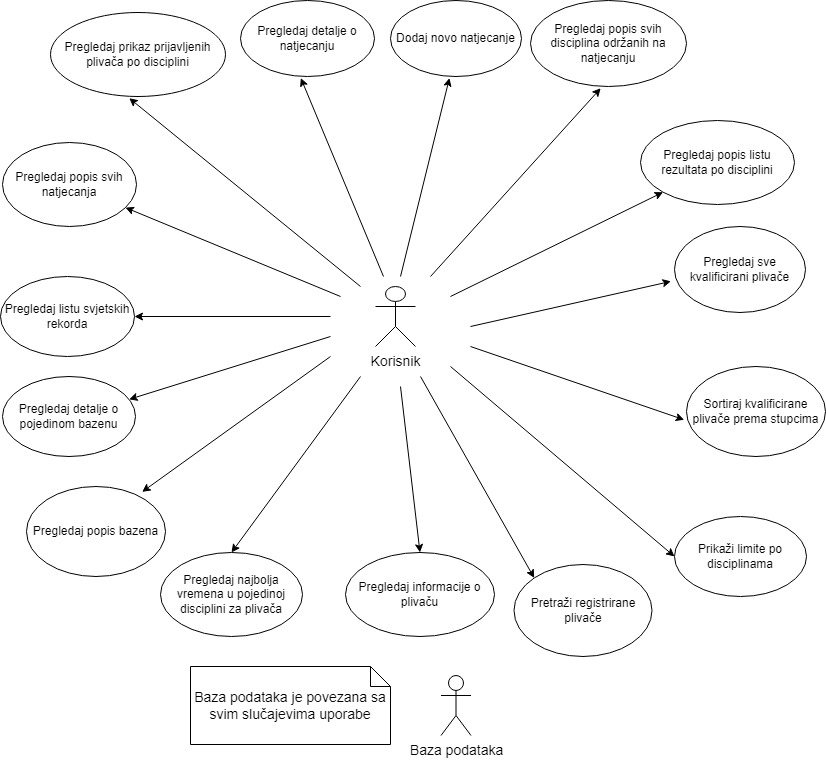
\includegraphics[width=\dimexpr\paperwidth-2cm,height=\paperheight,keepaspectratio]{usecase2.jpg}
    \centering
    \caption{Dijagram obazaca uporabe}
    \label{fig:use-case}
\end{figure}

\clearpage
\section{Opis obrazaca uporabe}

\begin{enumerate}
    \item Pregledaj popis svih natjecanju
    \begin{itemize}
        \item[$\bullet$] \textbf{Glavni sudionik:} Korisnik.
        \item[$\bullet$] \textbf{Cilj:} Pregledati popis svih natjecanja.
        \item[$\bullet$] \textbf{Ostali sudionici:} Baza podataka.
        \item[$\bullet$] \textbf{Preduvjeti:} Uspostavljena veza s internetom, podaci upisani u bazu, poslužitelj dostupan
        \item[$\bullet$] \textbf{Željeni scenarij:} Korisnik odabire stranicu s prikazom natjecanja i uspješno pregledava popis svih natjecanja.
        \item[$\bullet$] \textbf{Mogući ostali scenariji:} Podaci o natjecanjima nisu uneseni u bazu, ne prikazuju se korisniku.
    \end{itemize}



    \item Pregledaj prikaz prijavljenih plivača po disciplini 
    \begin{itemize}
        \item[$\bullet$] \textbf{Glavni sudionik:} Korisnik.
        \item[$\bullet$] \textbf{Cilj:} Pregledati popis broj prijavljenih plivača po disciplini.
        \item[$\bullet$] \textbf{Ostali sudionici:} Baza podataka.
        \item[$\bullet$] \textbf{Preduvjeti:} Uspostavljena veza s internetom, podaci upisani u bazu, poslužitelj dostupan.
        \item[$\bullet$] \textbf{Željeni scenarij:} Korisnik odabire ikonu s dijagramom na kartici s prikazom natjecanja i 
        uspješno pregledava stupčasti dijagram s brojem prijavljenih plivača po disciplini.
        \item[$\bullet$] \textbf{Mogući ostali scenariji:} Podaci o natjecanjima nisu uneseni u bazu, ne prikazuju se korisniku.
    \end{itemize}



    \item Pregledaj detalje o natjecanju
    \begin{itemize}
        \item[$\bullet$] \textbf{Glavni sudionik:} Korisnik.
        \item[$\bullet$] \textbf{Cilj:} Pregledati detalje o pojedinom natjecanja.
        \item[$\bullet$] \textbf{Ostali sudionici:} Baza podataka.
        \item[$\bullet$] \textbf{Preduvjeti:} Uspostavljena veza s internetom, podaci upisani u bazu, poslužitelj dostupan.
        \item[$\bullet$] \textbf{Željeni scenarij:} Korisnik odabire karticu s prikazom natjecanja i uspješno pregledava detalje o pojedinom natjecanja.
        \item[$\bullet$] \textbf{Mogući ostali scenariji:} Podaci o natjecanjima nisu uneseni u bazu, ne prikazuju se korisniku.
    \end{itemize}



    \item Dodaj novo natjecanje
    \begin{itemize}
        \item[$\bullet$] \textbf{Glavni sudionik:} Korisnik.
        \item[$\bullet$] \textbf{Cilj:} Dodati novo natjecanje na popis svih natjecanja.
        \item[$\bullet$] \textbf{Ostali sudionici:} Baza podataka.
        \item[$\bullet$] \textbf{Preduvjeti:} Uspostavljena veza s internetom, podaci upisani u bazu, poslužitelj dostupan.
        \item[$\bullet$] \textbf{Željeni scenarij:} Pritiskom na gumb s plusom, prikazuje se obrazac za dodavanje novog natjecanja. Korisnik popunjava podatke
        o novom natjecanju. Korisnik odabire opciju \textit{Save}. Novo natjecanje se prikazuje na popisu svih natjecanja
        \item[$\bullet$] \textbf{Mogući ostali scenariji:} Uneseni podaci su neispravni ili uneseni u nesipravnom formatu. 
        Korisniku se prikazuje poruka o greški prilikom validacije
    \end{itemize}


    \item Pregledaj popis svih disciplina održanih na natjecanju
    \begin{itemize}
        \item[$\bullet$] \textbf{Glavni sudionik:} Korisnik.
        \item[$\bullet$] \textbf{Cilj:} Pregledati popis svih disciplina održanih na natjecanju.
        \item[$\bullet$] \textbf{Ostali sudionici:} Baza podataka.
        \item[$\bullet$] \textbf{Preduvjeti:} Uspostavljena veza s internetom, podaci upisani u bazu, poslužitelj dostupan.
        \item[$\bullet$] \textbf{Željeni scenarij:} Pritiskom na ikonu s dokumentom na kartici odabranom natjecanja korisnika se preusmjerava na stranicu o odabranom
        natjecanju. Korisniku se prikazuju podaci o odabranom natjecanju i popis održanih disicplina.
        \item[$\bullet$] \textbf{Mogući ostali scenariji:} Rezultati natjecanja nisu uneseni u bazu, ne prikazuju se korisniku.
    \end{itemize}


    \item Pregledaj listu rezultata po disciplini
    \begin{itemize}
        \item[$\bullet$] \textbf{Glavni sudionik:} Korisnik.
        \item[$\bullet$] \textbf{Cilj:} Pregledati poredak plivača po disciplini
        \item[$\bullet$] \textbf{Ostali sudionici:} Baza podataka.
        \item[$\bullet$] \textbf{Preduvjeti:} Uspostavljena veza s internetom, podaci upisani u bazu, poslužitelj dostupan.
        \item[$\bullet$] \textbf{Željeni scenarij:} Pritiskom na pojedinu disciplinu prikazuje se gumb \textit{Event Results}. Klikom na prikazani gumb otvara
        se dijalog s poretkom plivača u odabranoj disciplini na odabranom natjecanju.
        \item[$\bullet$] \textbf{Mogući ostali scenariji:} Rezultati natjecanja nisu uneseni u bazu, ne prikazuju se korisniku.
    \end{itemize}


    \item Pregledaj sve kvalificirane plivače
    \begin{itemize}
        \item[$\bullet$] \textbf{Glavni sudionik:} Korisnik.
        \item[$\bullet$] \textbf{Cilj:} Pregledati sve kvalificirane plivače za Državno PH 2023.
        \item[$\bullet$] \textbf{Ostali sudionici:} Baza podataka.
        \item[$\bullet$] \textbf{Preduvjeti:} Uspostavljena veza s internetom, podaci upisani u bazu, poslužitelj dostupan.
        \item[$\bullet$] \textbf{Željeni scenarij:} Korisnik odabre karticu s prikazom kvalificiranih plivača za Državno PH. Korisniku se prikazuje
        lista svih plivača koji su otplivali zadane limite.
        \item[$\bullet$] \textbf{Mogući ostali scenariji:} Limiti ili plivači nisu uneseni u bazu, ne prikazuju se korisniku.
    \end{itemize}


    \item Poredaj kvalificirane plivače prema stupcima
    \begin{itemize}
        \item[$\bullet$] \textbf{Glavni sudionik:} Korisnik.
        \item[$\bullet$] \textbf{Cilj:} Poredati kvalificirane plivače prema stupcima.
        \item[$\bullet$] \textbf{Ostali sudionici:} Baza podataka.
        \item[$\bullet$] \textbf{Preduvjeti:} Uspostavljena veza s internetom, podaci upisani u bazu, poslužitelj dostupan.
        \item[$\bullet$] \textbf{Željeni scenarij:} Korisnik pritiskom na pojedini stupac odabire različite mogućnosti poretka.
        \item[$\bullet$] \textbf{Mogući ostali scenariji:} Podaci nisu uneseni u bazu, ne prikazuju se korisniku.
    \end{itemize}


    \item Prikaži limite po disciplinama
    \begin{itemize}
        \item[$\bullet$] \textbf{Glavni sudionik:} Korisnik.
        \item[$\bullet$] \textbf{Cilj:} Pregledati limiti po disciplinama.
        \item[$\bullet$] \textbf{Ostali sudionici:} Baza podataka.
        \item[$\bullet$] \textbf{Preduvjeti:} Uspostavljena veza s internetom, podaci upisani u bazu, poslužitelj dostupan.
        \item[$\bullet$] \textbf{Željeni scenarij:} Korisniki se pritiskom na gumb \textit{Qualifying Standards} na dnu stranicu prikazuje
        popis svih limita u dvije liste: jedna prikazuje limite u muškoj kategoriji, a druga limite u ženoskoj kategoriji.
        \item[$\bullet$] \textbf{Mogući ostali scenariji:} Podaci nisu uneseni u bazu, ne prikazuju se korisniku.
    \end{itemize}


    \item Pretraži registrirane plivače
    \begin{itemize}
        \item[$\bullet$] \textbf{Glavni sudionik:} Korisnik.
        \item[$\bullet$] \textbf{Cilj:} Pretražiti registrirane plivače.
        \item[$\bullet$] \textbf{Ostali sudionici:} Baza podataka.
        \item[$\bullet$] \textbf{Preduvjeti:} Uspostavljena veza s internetom, podaci upisani u bazu, poslužitelj dostupan.
        \item[$\bullet$] \textbf{Željeni scenarij:} Korisnik odabire stranicu s prikazom polja za pretraživanje plivača. Korisniku unosi puno
        ime i prezime željenog plivača i odabire opciju prikaza pritiskom na gumb \textit{Search}. Korisniku se prikazuje starnica s prikazom detalja o
        željenom plivaču.
        \item[$\bullet$] \textbf{Mogući ostali scenariji:} 
        \begin{enumerate}
            \item Uneseno ime i prezime ne postoji u bazi, korisnika se ne preusmjerava na stranicu o plivaču.
            \item Korisnik nema rezultata u bazi, ne prikazuje se lista najboljih rezultata.
        \end{enumerate}
    \end{itemize}


    \item Pretraži podatke o registriranom plivaču
    \begin{itemize}
        \item[$\bullet$] \textbf{Glavni sudionik:} Korisnik.
        \item[$\bullet$] \textbf{Cilj:} Pregledati inforamcije o registriranom plivaču
        \item[$\bullet$] \textbf{Ostali sudionici:} Baza podataka.
        \item[$\bullet$] \textbf{Preduvjeti:} Uspostavljena veza s internetom, podaci upisani u bazu, poslužitelj dostupan. 
        Korisnik je unio ispravno ime i prezime plivača na stranici za pretraživanje registriranih plivača.
        \item[$\bullet$] \textbf{Željeni scenarij:} Korisniku se prikazuje stranica
        s informacijama o željenom plivaču i listom njegovih najboljih rezultata u pojedinoj disciplini.
        \item[$\bullet$] \textbf{Mogući ostali scenariji:} Podaci o plivaču nisu uneseni u bazu, ne prikazuju se njegovi najbolji rezultati.
    \end{itemize}

    \item Pregledaj popis bazena
    \begin{itemize}
        \item[$\bullet$] \textbf{Glavni sudionik:} Korisnik.
        \item[$\bullet$] \textbf{Cilj:} Pregledati popis svih bazena. 
        \item[$\bullet$] \textbf{Ostali sudionici:} Baza podataka.
        \item[$\bullet$] \textbf{Preduvjeti:} Uspostavljena veza s internetom, podaci upisani u bazu, poslužitelj dostupan.
        \item[$\bullet$] \textbf{Željeni scenarij:} Korisnik odabire stranicu s prikazom svih bazena. Korisniku se prikazuje popis bazena
        unesenih u bazu.
        \item[$\bullet$] \textbf{Mogući ostali scenariji:} Podaci nisu uneseni u bazu, ne prikazuju se korisniku.
    \end{itemize}
    
    \item Pregledaj detalje o bazenu
    \begin{itemize}
        \item[$\bullet$] \textbf{Glavni sudionik:} Korisnik.
        \item[$\bullet$] \textbf{Cilj:} Pregledati detalje o pojedinom bazenu.
        \item[$\bullet$] \textbf{Ostali sudionici:} Baza podataka.
        \item[$\bullet$] \textbf{Preduvjeti:} Uspostavljena veza s internetom, podaci upisani u bazu, poslužitelj dostupan.
        \item[$\bullet$] \textbf{Željeni scenarij:} Korisnik odabire karticu s prikazom bazena i uspješno pregledava detalje o odabranom bazenu.
        \item[$\bullet$] \textbf{Mogući ostali scenariji:} Podaci o bazenu nisu uneseni u bazu, ne prikazuju se korisniku.
    \end{itemize}

    \item Pregledaj listu svjetskih rekorda
    \begin{itemize}
        \item[$\bullet$] \textbf{Glavni sudionik:} Korisnik.
        \item[$\bullet$] \textbf{Cilj:} Pregledati listu trenutnih svjetskih rekorda.
        \item[$\bullet$] \textbf{Ostali sudionici:} Baza podataka.
        \item[$\bullet$] \textbf{Preduvjeti:} Uspostavljena veza s internetom, podaci upisani u bazu, poslužitelj dostupan
        \item[$\bullet$] \textbf{Željeni scenarij:} Korisnik odabire stranicu s prikazom svjetskih rekorda. Korisniku se prikazuju trenutni svjetski rekordi
        u pojedinoj disciplini u muškoj i ženskoj kategoriji.
        \item[$\bullet$] \textbf{Mogući ostali scenariji:} Podaci o svjtskim rekordima nisu uneseni u bazu, ne prikazuju se korisniku.
    \end{itemize}

\end{enumerate}

\chapter{Baza podataka}

\section{Korištene tehnologije}
U ovom projektu korištene su dvije ključne tehnologije, DBeaver i PostgreSQL baza podataka, koje su omogućile
učinkovito upravljanje podacima.

\subsection{DBeaver}
DBeaver je popularan alat za upravljanje bazama podataka koji pruža intuitivno korisničko sučelje i 
podršku za različite baze podataka, uključujući PostgreSQL.
Odabir DBeavera omogućio je jednostavno povezivanje s bazom podataka, 
brzo izvršavanje upita i efikasno upravljanje shemom baze podataka.

\subsection{PostgreSQL}
PostgreSQL je otvorena i objektno-relacijska baza podataka koja je odabrana za ovaj projekt iz nekoliko razloga. 
Prvo, PostgreSQL pruža napredne mogućnosti za upravljanje podacima, uključujući podršku za kompleksne upite, transakcije i indeksiranje. 
Također nudi visoku razinu pouzdanosti, što je važno za ovu aplikaciju za praćenje plivačkih rezultata.

\clearpage

\section{ER Model}
ER model \engl{Entity-relationship model} baze podataka je konceptualni alat koji nam pomaže organizirati i prikazati strukturu podataka na intuitivan način. 
U ER modelu koristimo entitete koji predstavljaju stvari ili koncepte u stvarnom svijetu, kao što su korisnici, proizvodi ili narudžbe. 
Svaki entitet ima svoje atribute koji opisuju karakteristike tog entiteta, poput imena, adrese ili cijene. 
Osim toga, ER model koristi veze između entiteta kako bi prikazao njihove međusobne odnose, kao što su veze "ima" ili "pripada". 
Korištenjem ER modela, možemo bolje razumjeti strukturu podataka.

\vspace{\baselineskip}

\subsection{Opis ER modela}

Podaci spremljeni u ovoj bazi uključuju informacije o plivačima(osobama), plivačkim natjecanjima, plivačkim bazenima, plivačkim rezultatima, limitima i svjetskim rekordima.

\vspace{\baselineskip}

Središnji entitet ove baze je entitet rezultat jer se cijeli prikaz podataka temelji na rezultatima. Entitet rezultat predstavlja jedinstveno isplivano vrijeme određenog plivača
u određenoj disciplini na određenom natjecanju. Zbog toga su veze \textit{jeOtplivao}, \textit{jeDiscipline} i \textit{jeIsplivanNa} oblika 1:N. 

\vspace{\baselineskip}

Za plivača se uz osnovne podatke osobi bilježi i država koju predstavlja te klub za koji nastupa. Klub ima prijavljen matični bazen na kojemu održava svoje treninge.
Bazen uz osnovne podatke o bazenu ima i podatke o mjestu na kojem se nalazi, tj. Državi u kojoj se nalazi. Natjecanje se održava na točno određenom bazenu.

\vspace{\baselineskip}

Discipline su sve moguće pojedinačne discipline u muškoj i ženskoj kategoriji. Za svaku disciplinu se bilježi trenutni svjetski rekord i limit koji je potrebno isplivati
za nastup na Državnom PH 2023. ER model je prikazan na slici \ref*{fig:ER model}.

\clearpage

\begin{figure}[!h]
    \centering
    \hspace*{-2.5cm}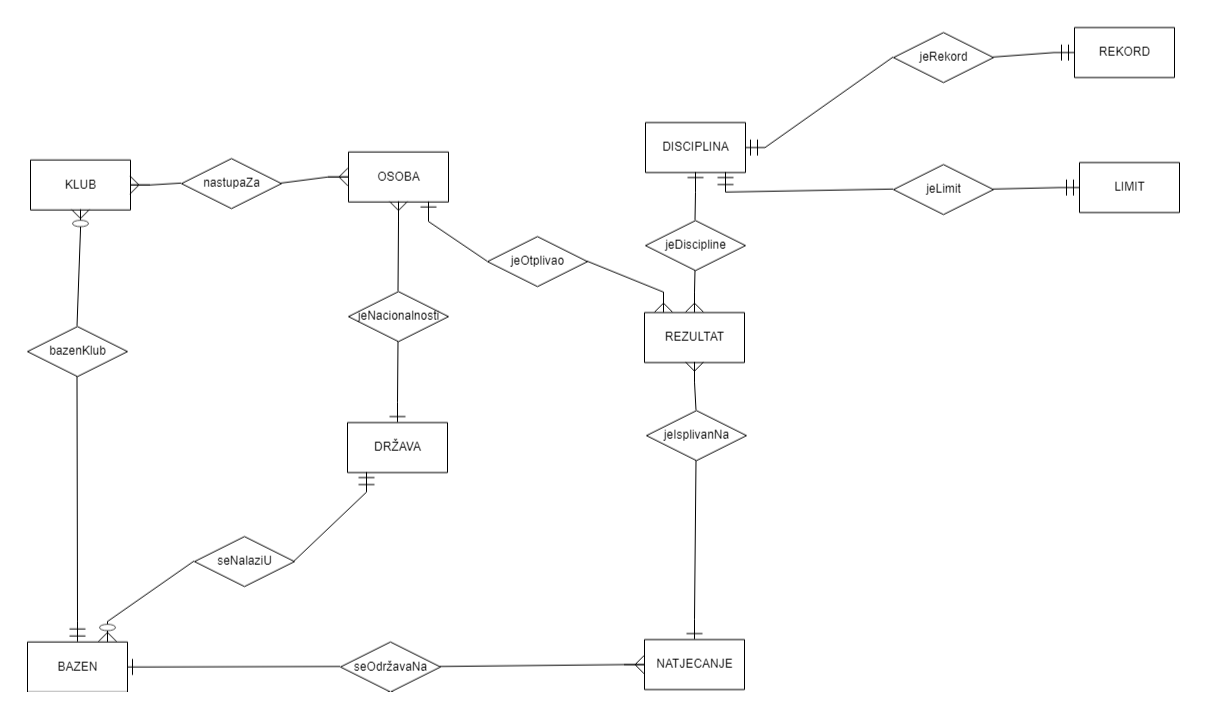
\includegraphics[width=\dimexpr\paperwidth-2cm,height=\paperheight,keepaspectratio]{ER model.png}
    \centering
    \caption{ER model baze podataka}
    \label{fig:ER model}
\end{figure}

\subsection{Popis entiteta i atributa}

\vspace{\baselineskip}

\textbf{OSOBA} - \underline{idosoba}, imeosoba, prezimeosoba, spol, datumrodjenja, visina, tezina, \dashuline{idklub}, \dashuline{iddrzava}

\vspace{\baselineskip}

\textbf{REZULTAT} - \underline{idrezultat}, vrijme, bodovi, datum, idosoba, iddisciplina, idnatjecanje

\vspace{\baselineskip}

\textbf{NATJECANJE} - \underline{idnatjecanje}, nazivnatjecanje, vrstanatjecanje, datumod, datumdo, \\
\indent idbazen

\vspace{\baselineskip}

\textbf{BAZEN} - \underline{idbazen}, nazivbazen, kapacitet, grad, adresa, iddrzava

\vspace{\baselineskip}

\textbf{KLUB} - \underline{idklub}, nazivglub, godinaosnivanja, idbazen

\vspace{\baselineskip}

\textbf{DISCIPLINA} - \underline{iddisciplina}, nazivdisciplina, spol

\vspace{\baselineskip}

\textbf{DRZAVA} - \underline{iddrzava}, nazivdrzava

\vspace{\baselineskip}

\textbf{LIMIT} - \underline{idlimit}, vrijeme, iddisciplina

\vspace{\baselineskip}

\textbf{REKORD} - \underline{idrekord}, vrijeme, iddisciplina

\vspace{\baselineskip}

Napomena: Primarni ključevi podvučeni su punom linijom.

\subsection{Popis veza}

\vspace{\baselineskip}

\textbf{jeOtplivao} - \underline{idrezultat}, idosoba

\vspace{\baselineskip}

\textbf{jeIsplivanNa} - \underline{idrezultat}, idnatjecanje

\vspace{\baselineskip}

\textbf{nastupaZa} - \underline{idosoba}, idklub

\vspace{\baselineskip}

\textbf{jeNacionalnosti} - \underline{idosoba}, iddrzava

\vspace{\baselineskip}

\textbf{bazenKlub} - \underline{idbazen}, idklub

\vspace{\baselineskip}

\textbf{seNalaziU} - \underline{idbazen}, iddrzava 

\vspace{\baselineskip}

\textbf{jeDiscipline} - \underline{idrezultat}, iddisciplina

\vspace{\baselineskip}

\textbf{jeLimit} - \underline{iddisciplina}, idlimit 

\vspace{\baselineskip}

\textbf{jeRekord} - \underline{iddisciplina}, idrekord

\vspace{\baselineskip}

Napomena: Primarni ključevi podvučeni su punom linijom.

\vspace{\baselineskip}


\section{Relacijski model}

\subsection{Preslikavanje ER modela u relacijski model baze podataka}

Prikazani ER model preslikat će se u relacijski model PostgreSQL baze podataka. Strani ključevi nastaju na temelju
N:1 prikazanih veza u kojima se primarni ključ sastoji od jednog atributa. Relacijski model baze podataka prikazan je
na slici \ref{fig:relacijski model}.

\subsection{Popis relacija}

\vspace{\baselineskip}

Relacijski model sastoji se od navedenih relacija:

\vspace{\baselineskip}

\begin{itemize}
    \item[$\bullet$] \textbf{OSOBA} - \underline{idosoba}, imeosoba, prezimeosoba, spol, datumrodjenja, visina, tezina, 
    \dashuline{idklub}, \dashuline{iddrzava} \\
    Relacija 'Osoba' sadrži primarni ključ koji jednoznačno identificira svaku osobu. U relaciju se uz idosobe spremaju: ime osobe, prezime osobe,
    spol, datum rođenja, visina i težina. Atribut 'idklub' je strani ključ koji referencira relaciju 'Klub' te predstavlja klub za koji plivač nastupa.
    Atribut 'iddrzava' je strani ključ koji referencira relaciju 'Država' te predstavlja državu koju plivač predstavlja na natjecanjima.
    
\vspace{\baselineskip}

    \item[$\bullet$] \textbf{REZULTAT} - \underline{idrezultat}, vrijme, bodovi, datum, idosoba, iddisciplina, idnatjecanje,
    \dashuline{iddisciplina}, \dashuline{idnatjecanje}, \dashuline{idosoba} \\
    Relacija 'Rezultat' sadrži primarni ključ koji jednoznačno identificira svaki rezultat pohranjen u bazi. U relaciju se spremaju vrijeme rezultata, 
    bodovi (izračunati u odnosu na svjetski rekord), datum na koji je rezultat isplivan. Relacija sadrži tri strana ključa. Atribut 'idosoba' je strani ključ
    koj referencira relaciju 'Osoba' i predstavlja osobu koja je isplivala rezultat. Atribut 'iddisciplina' je strani ključ
    koj referencira relaciju 'Disciplina' i predstavlja disciplinu u kojoj je rezultat isplivan. Atribut 'idnatjecanje' je strani ključ
    koj referencira relaciju 'Natjecanje' i predstavlja natjecanje na kojem je rezultat isplivan.

\vspace{\baselineskip}

    \item[$\bullet$] \textbf{NATJECANJE} - \underline{idnatjecanje}, nazivnatjecanje, vrstanatjecanje, datumod, datumdo, \dashuline{idbazen} \\
    Relacija 'Natjecanje' sadrži primarni ključ 'idnatjecanje' koji jednoznačno identificira svako natjecanje. Ostali atributi u relaciji su naziv natjecanja, 
    vrsta natjecanja - koja se odnosi na olimpijske igre, svjetsko prventsvo,...Uz ove atribute bilježi si datum početka i datum završetka natjecnaja.
    Atribut 'idbazen' je strani ključ koji referencira relaciju 'Bazen' i predstavlja bazen na kojem se natjecanje održava.

\vspace{\baselineskip}

    \item[$\bullet$] \textbf{BAZEN} - \underline{idbazen}, nazivbazen, kapacitet, grad, adresa, \dashuline{iddrzava} \\
    Relacija 'Bazen' predstavlja registrirane olimpijske bazene i sadrži primarni ključ 'idbazen'. U relaciju se pohranjuje naziv bazena, kapacitet ljudi 
    koji mogu pristupiti bazene te grad i adresa na kojoj se bazen nalazi. Atribut 'iddrzava' je strani ključ koji predstavlja državu u kojoj se bazen nalazi i 
    referencira relaciju 'Država'.

\vspace{\baselineskip}

    \item[$\bullet$] \textbf{KLUB} - \underline{idklub}, nazivglub, godinaosnivanja, \dashuline{idbazen} \\
    Relacija 'Klub' predstavlja prijavljene klubove koji sudjeluju na natjecanjima. Atribut 'idklub' je primarni ključ. Ostali atributi u relaciji predstavljaju
    podatke od nazivu klub i godini osnivanja kluba. Atribut 'idbazen' je strani ključ koji referencira relaciju 'Bazen' i predstavlja matični bazen kluba na kojemu
    se održavaju treninzi. 

\vspace{\baselineskip}

    \item[$\bullet$] \textbf{DISCIPLINA} - \underline{iddisciplina}, nazivdisciplina, spol \\
    U relaciju 'Disciplina' pohranjuju se podaci o svim mogućim pojedinačnim disciplinama, dakle 50m, 100m, 200m u svakom stilu (slobodno, leđno, prsno i leptir) i posebno u
    muškoj i ženskoj kategoriji te 400, 800 i 1500 slobodno, 200 i 400 mješovito. Dakle atribut 'iddisciplina' je primarni ključ, a naziv discipline je jedan od navedenih u kombinaciji
    sa spolom.

\vspace{\baselineskip}

    \item[$\bullet$] \textbf{DRZAVA} - \underline{iddrzava}, nazivdrzava \\
    U relaciji 'Država' pohranjuju se nazivi države uz primarni ključ na osnovi atributa 'iddrzava' koji je primarni ključ.

\vspace{\baselineskip}

    \item[$\bullet$] \textbf{LIMITI} - \underline{idlimit}, vrijeme, \dashuline{iddisciplina} \\
    U relaciji 'Limiti' pohranjuju se limiti koje je potrebno isplivati za nastup na Državnom PH 2023. Atribut 'idlimit' je primarni ključ, a 'iddisciplina' 
    je strani ključ koji referencira relaciju 'Disciplina'. Vrijeme je vrijeme limita. 

\vspace{\baselineskip}

    \item[$\bullet$] \textbf{REKORD} - \underline{idrekord}, vrijeme, \dashuline{iddisciplina} \\
    U relaciji 'Rekord' pohranjuju se svjetski rekordi, dakle najbrža vremena u svakoj disciplini u muškoj i ženskoj kategoriji. Atribut 'idlimit' je primarni ključ, 
    a 'iddisciplina' je strani ključ koji referencira relaciju 'Disciplina'. Vrijeme je vrijeme svjetskog rekorda. 
    
\end{itemize}

Napomena: Primarni ključevi podvučeni su punom linijom, \\
\indent a strani ključevi isprekidanom linijom.

\begin{figure}[htb]
    \centering
    \hspace*{-2.5cm}
    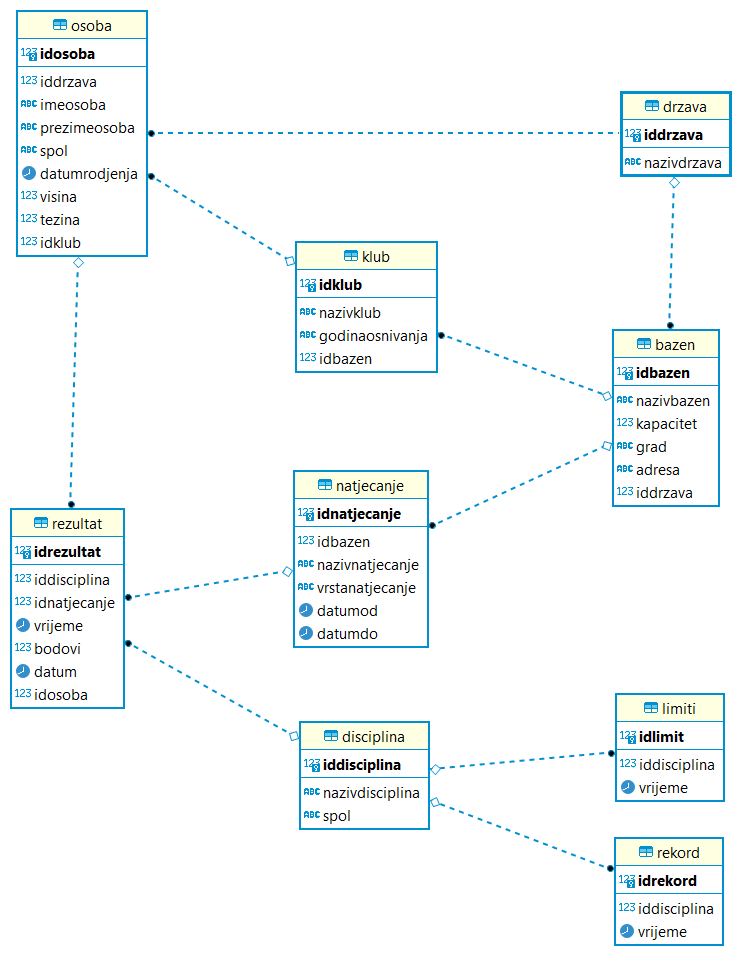
\includegraphics[width=\dimexpr\paperwidth-5cm,height=\paperheight-5cm,keepaspectratio]{Relacijski model.png}
    \centering
    \caption{Relacijski model baze podataka}
    \label{fig:relacijski model}
\end{figure}

\section{Stvaranje baze podataka}
U nastavku slijede neke od SQL naredbi za kreiranje relacija baze podataka:

\begin{lstlisting}
    CREATE TABLE IF NOT EXISTS osoba (
        idosoba SERIAL PRIMARY KEY,
        imeosoba VARCHAR,
        prezimeosoba VARCHAR,
        spol VARCHAR,
        datumrodjenja DATE,
        visina NUMERIC(5, 2),
        tezina NUMERIC(5, 2),
        idklub INT,
        iddrzava INT,
        FOREIGN KEY (idklub) REFERENCES klub (idklub),
        FOREIGN KEY (iddrzava) REFERENCES drzava (iddrzava)
    );

    CREATE TABLE rezultat (
        idrezultat SERIAL PRIMARY KEY,
        vrijeme TIMESTAMP(3) WITHOUT TIME ZONE,
        bodovi INT,
        datum DATE,
        idosoba INT,
        iddisciplina INT,
        idnatjecanje INT,
        FOREIGN KEY (idosoba) REFERENCES osoba (idosoba),
        FOREIGN KEY (iddisciplina) REFERENCES disciplina (iddisciplina),
        FOREIGN KEY (idnatjecanje) REFERENCES natjecanje (idnatjecanje)
    );

    CREATE TABLE natjecanje (
        idnatjecanje SERIAL PRIMARY KEY,
        nazivnatjecanje VARCHAR,
        vrstanatjecanje VARCHAR,
        datumod DATE,
        datumdo DATE,
        FOREIGN KEY (idbazen) REFERENCES bazen (idbazen)
        idbazen INT,
    );



\end{lstlisting}

\section{Popunjavanje baze podataka}
U nastavku slijede neke od INSERT SQL naredbi za popunjavanje baze podataka podacima.

\begin{lstlisting}
    INSERT INTO osoba (idosoba, iddrzava, imeosoba, prezimeosoba, spol, datumrodjenja, visina, tezina)
    VALUES 
    ( (SELECT iddrzava FROM drzava WHERE nazivdrzava = 'Croatia'), 'Leo',  'Sudar', 'M', '1998-02-21', 182, 81, 4),
    ( (SELECT iddrzava FROM drzava WHERE nazivdrzava = 'Croatia'), 'Ivano',  'Petrovi', 'M', '1995-11-14', 185, 98, 9),
    ( (SELECT iddrzava FROM drzava WHERE nazivdrzava = 'Croatia'), 'Lovro',  'Tomi', 'M', '1998-09-09', 168, 89, 1),
    ( (SELECT iddrzava FROM drzava WHERE nazivdrzava = 'Croatia'), 'Nino',  'Lovri', 'M', '1992-06-27', 170, 91, 9),
    ( (SELECT iddrzava FROM drzava WHERE nazivdrzava = 'Croatia'), 'Marko',  'Radi', 'M', '2000-09-24', 177, 82, 6),
    ( (SELECT iddrzava FROM drzava WHERE nazivdrzava = 'Croatia'), 'Dario',  'Peri', 'M', '2004-11-29', 181, 91, 9),


    INSERT INTO rezultat (idrezultat, vrijeme, bodovi, datum, iddisciplina, idnatjecanje, idosoba)
    VALUES 
    (2055, 1, 15, '1970-01-01 00:00:29.419', 710, '2022-11-12', 97),
    (2056, 1, 15, '1970-01-01 00:00:25.479', 820, '2022-11-12', 51),
    (2057, 1, 15, '1970-01-01 00:00:25.622', 816, '2022-11-12', 133),
    (2058, 1, 15, '1970-01-01 00:00:25.150', 831, '2022-11-12', 154),
    (2059, 1, 15, '1970-01-01 00:00:27.246', 767, '2022-11-12', 106),
    (2060, 1, 15, '1970-01-01 00:00:26.855', 778, '2022-11-12', 60),
    (2064, 1, 15, '1970-01-01 00:00:29.847', 700, '2022-11-12', 143);


    INSERT INTO rekordi (idrekord, iddisciplina, vrijeme)
    VALUES
    (1, 1, '00:00:20.910'),
    (2, 2, '00:00:23.670'),
    (3, 3, '00:00:46.860'),
    (4, 4, '00:00:51.710'),
    (5, 5, '00:01:42.000'),  
    (6, 6, '00:01:52.980'),
    (7, 7, '00:03:40.070'),


\end{lstlisting}

\chapter{Web aplikacija}

\section{Korištene tehnologije}

\subsection{Java Spring i JPA}
Java Spring je popularni okvir za razvoj web aplikacija koji olakšava izgradnju pouzdanih i skalabilnih aplikacija. 
Koristeći koncepte poput inversije upravljanja i ubrizgavanja ovisnosti, programeri mogu efikasno razvijati i testirati aplikacije. 
JPA (Java Persistence API) je standardna Java specifikacija koja omogućava upravljanje podacima u bazama podataka. 
Kombinacija Springa i JPA-e olakšava mapiranje Java objekata na bazu podataka i izvršavanje osnovnih operacija nad podacima.

\subsection{Vue.js}
Vue.js je moderni JavaScript okvir koji se koristi za izgradnju korisničkih sučelja te
pruža modularnost, reaktivnost i jednostavnu integraciju s drugim alatima. 
Uspoređujući s običnim JavaScriptom, Vue.js omogućava brži razvoj aplikacija s manje koda i pruža bogat ekosustav resursa za podršku.

Sastoji se od tri glavna dijela: HTML, CSS i JavaScript.

\begin{itemize}

    \item[$\bullet$]HTML: Vue.js koristi HTML za definiranje strukture korisničkog sučelja. 
    Korisnik definira elemente kao što su gumbi i forme koji će se prikazivati.

    \item[$\bullet$]CSS: CSS se koristi za definiranje izgleda i stila elemenata u Vue.js aplikacijama. 
    Korisnik može primijeniti različite stilove, boje, margine i druge stilizacijske atribute kako bi prilagodio izgled korisničkog sučelja.

    \item[$\bullet$]JavaScript: JavaScript je jezik koji se koristi za definiranje interaktivnosti i logike u Vue.js aplikacijama. 
    Korisnik može koristiti JavaScript kako bi reagirao na događaje korisnika, upravljao podacima i izvršavao različite operacije.

\end{itemize}

\subsection{Vuetify 3}
Vuetify je napredna biblioteka komponenti za Vue.js koja olakšava izradu modernih korisničkih sučelja. 
Sadrži bogat skup gotovih komponenti kao što su tipografija, gumbi, forme, tablice i mnoge druge.
Koristi se za izradu intuitivnog dizajna i popularan je za izgradnju atraktivnih i responzivnih web aplikacija.


\section{MVC obrazac}
MVC (Model-View-Controller) arhitektura je popularan koncept koji se koristi u razvoju aplikacija kako bi se postigla bolja organizacija i razdvajanje odgovornosti. 
Ova arhitektura se temelji na ideji podjele aplikacije na tri glavna dijela: Model, Pogled i Nadglednik. 
Svaki od tih dijelova ima specifičnu ulogu i zajedno stvaraju cjelovitu aplikaciju.

\vspace{\baselineskip}

MVC arhitektura omogućava bolje upravljanje i organizaciju aplikacija kroz sljedeće glavne značajke:


\begin{enumerate}
    
    \item Model:
    \begin{itemize}
        \item[$\bullet$] Model predstavlja poslovne podatke i logiku aplikacije.
        \item[$\bullet$] Ovdje se čuvaju i obrađuju podaci te se izvršavaju operacije na njima.
        \item[$\bullet$] Model je odgovoran za interakciju s bazu podataka ili drugim izvorima podataka.
    \end{itemize}

    \item Pogled:
    \begin{itemize}
        \item[$\bullet$] Pogled predstavlja korisničko sučelje kroz koje korisnik komunicira s aplikacijom.
        \item[$\bullet$] Ovdje se prikazuju podaci iz Modela na korisnički prihvatljiv način.
        \item[$\bullet$] Pogled je odgovoran za prikazivanje podataka i reagiranje na korisničke akcije.
    \end{itemize}

    \item Nadglednik:
    \begin{itemize}
        \item[$\bullet$] Nadglednik upravlja logikom aplikacije i korisničkim zahtjevima.
        \item[$\bullet$] Prima ulazne podatke od korisnika putem Pogleda i obrađuje ih.
        \item[$\bullet$] Nadglednik ažurira Model s novim podacima i ažurira Pogled kako bi odražavao promjene.
    \end{itemize}

\end{enumerate}


\noindent Prednosti korištenja MVC arhitekture su:


\begin{itemize}
    \item[$\bullet$] Jasnija organizacija i struktura koda, što olakšava čitanje i održavanje aplikacije.
    \item[$\bullet$] Bolja razdvojenost odgovornosti između dijelova aplikacije, što olakšava izmjene i proširenja.
    \item[$\bullet$] Lakše testiranje jer se logika i prikaz odvajaju.
    \item[$\bullet$] Omogućava paralelni razvoj, jer timovi mogu istovremeno raditi na različitim dijelovima aplikacije.
    \item[$\bullet$] Poboljšava ponovnu upotrebu koda, jer se logika može koristiti s različitim prikazima.
\end{itemize}

\noindent Ukratko, MVC arhitektura pruža strukturu i organizaciju za razvoj aplikacija, olakšava održavanje, testiranje i proširenje.


\section{Arhitektura web aplikacije}

Web aplikacija za prikaz plivačkih rezultata i pregledavanje podataka o plivačkim natjecanjima koristi svoj MVC obrazac
za organizaciju arhitekture.

\subsection{Sloj podataka}
Sloj podataka sastoji se od dva dijela: razred Model (ili Entitet) i sučelje Repository.

\begin{enumerate}

    \item[$\textbf1.$] \textbf{Model} \\
    Za svaku relaciju u bazi podataka mora postojati određeni entitet u sloju podataka koji predstavlja tu relaciju i njene atribute.
    Pomoću tog modela vrši se mapiranje između privatnih članskih varijabli razreda Modela i atributa u tablici. Odsječak koda na slici
    \ref{fig:model} prikazuje model Natjecanja. Strani ključ je modeliran referencom na cijeli razred referencirajuće relacije. 

    \begin{figure}[!h]
        \centering
        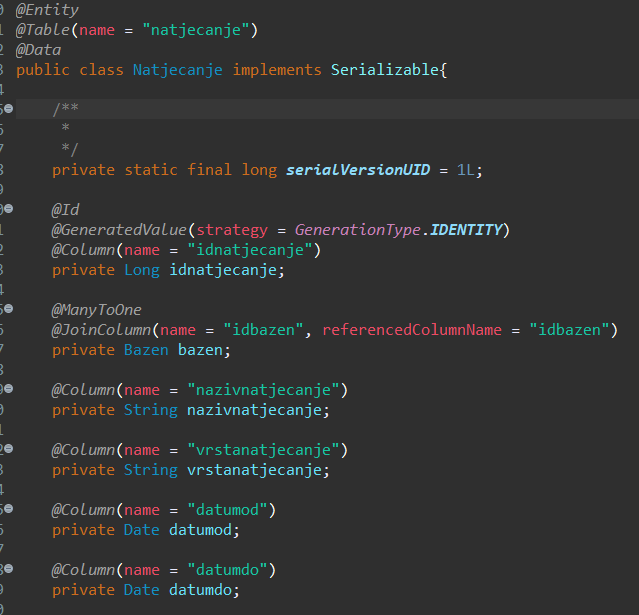
\includegraphics[width=10cm, height=10cm, keepaspectratio]{model.png}
        \centering
        \caption{Razred Natjecanje - model}
        \label{fig:model}
    \end{figure}

    \item[$\textbf2.$] \textbf{Repozitorij} \\
    Za svaki entitet definira se sučelje Repository koje nasljeđuje sučelje JpaRepository te time naasljeđuje i metode za dohvat
    podataka iz baze. JPA omogućuje pisanje SQL upita za dohvat podataka koristeći jednostavnu metodu imenovanja kojom u imenu metode
    definiramo po kojim atributima želimo da se upit vrši. Npr. Ako želimo dohvatiti natjecanje prema jedinstvenom 'idnatjecanje' 
    jednostavno definiramo metodu List<Natjecanje> findByIdnatjecanje(Long idnatjecanje) (prikazano na slici \ref{fig:repository}) koju koristimo u Kontroleru. 

    \begin{figure}[!h]
        \centering
        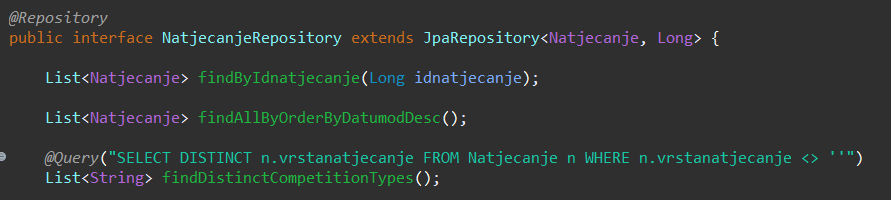
\includegraphics[width=15cm, height=10cm, keepaspectratio]{repository.png}
        \centering
        \caption{Sučelje NatjecanjeRepository - repozitorij}
        \label{fig:repository}
    \end{figure}

\end{enumerate}


\subsection{Sloj poslovne logike}

Kontroler \engl{Controller} je sloj koji se definira za svaki entitet Model i on obrađuje ulazne HTTP zahtjeve. Ovisno o dolaznom zahtjevu
odabire metodu koju će pozvati i tako vraća podatke. Na slici \ref{fig:controller} vidimo primjer Java Kontrolera s prikazom metoda
koje se nalaze svaka na svojoj putanji.

\begin{figure}[!h]
    \centering
    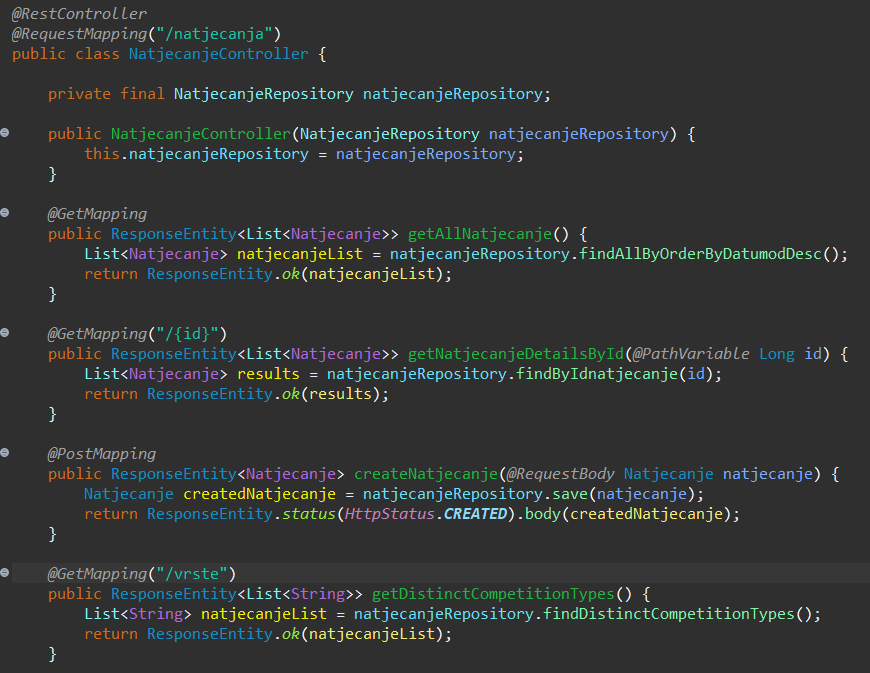
\includegraphics[width=15cm, height=10cm, keepaspectratio]{controller.png}
    \centering
    \caption{Razred NatjecanjeController - kontroler}
    \label{fig:controller}
\end{figure}

Drugi dio poslovne logike je ostvaren u Vue.js-u u JavaScriptu pomoću kojega se komunicira s kontrolerima na poslužiteljskoj strani.
Na slici \ref{fig:vue.js-api} je prikazan isječak koda u kojem se dohvaćaju podaci iz baze podataka na klijentsku stranu. 

\begin{figure}[!h]
    \centering
    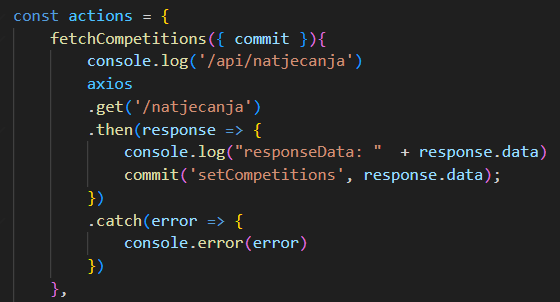
\includegraphics[width=10cm, height=10cm, keepaspectratio]{vue.js-api.png}
    \centering
    \caption{Vue.js akcija za dohvat podataka sa servera}
    \label{fig:vue.js-api}
\end{figure}

\subsection{Sloj korisničkog sučelja}
Ovo je sloj koji komunicira s korisnikom. Korisnik ne mora znati ništa o sloju podataka, niti o sloju poslovne logike da bi uspješno
koristio aplikaciju. Korisničko sučelje je izvedeno pomoću JavaScript radnog okvira Vue.js te se za gotove komponente i stilizacijske
elemenate koristi Vuetify biblioteka. Na slici \ref{fig:vue.js-component} je prikazan isječak koda jedne komponente za prikaz podataka korisnicima.

\begin{figure}[!h]
    \centering
    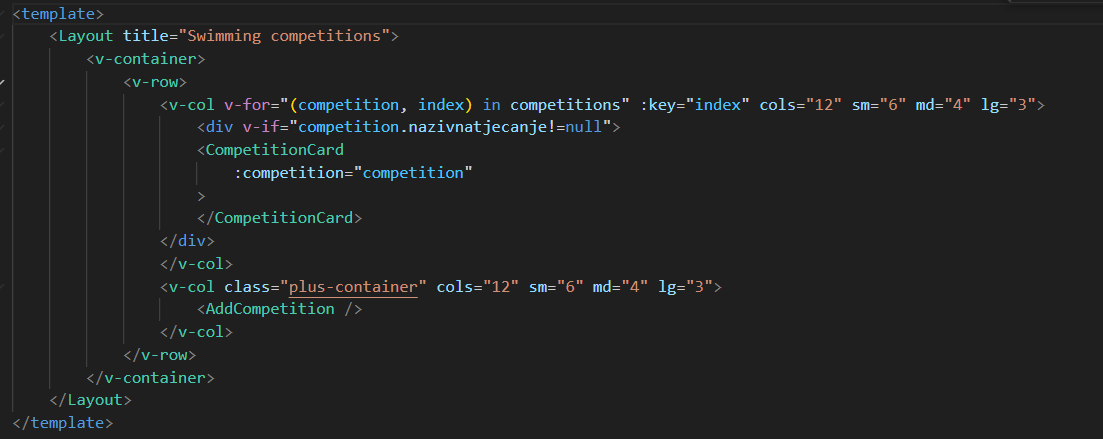
\includegraphics[width=15cm, height=10cm, keepaspectratio]{vue.js-component.png}
    \centering
    \caption{Vue.js komponenta za prikaza kartica natjecanja}
    \label{fig:vue.js-component}
\end{figure}


\chapter{Korisničke upute}

\section{Korisničko sučelje}
Korisničko sučelje omogućava pregled svih podataka o rezultatima, plivačima, limitima, bazenima i natjecanjima. \\
Nakon pokretanja aplikacije korisnik se nalazi na početnom zaslonu. Korisnik može odabrati druge stranice klikom na strelice
na lijevom i desnom uglu stranice. Korisnik također može koristiti navigacijsku traku za navigiranje kroz aplikaciju koja se prikazuje
klikom na gumb u gornjem desnom uglu stranice. Moguće opcije su redom: natjecanja, kvalificirani plivači, plivači, bazeni te svjetski rekordi.

\subsection{Natjecanja}
Odabirom kartice natjecanja prikazuju se sva registrirana natjecanja (slika \ref{fig:competition-add}). Korisnik na kartici za natjecanje može odabrati tri opcije:
\begin{enumerate}
    \item Ikona dokumenta - prikaz rezultata s natjecanja. Na ovoj stranici potrebno je odabrati željenu disciplinu i pritisnuti gumb
    'Rezultati discipline' da bi se prikazali svi rezultati u toj disciplini (slika \ref{fig:competition-details}).
    \item Ikona grafa - prikaz stupčastog dijagrama prijavljenih plivača za natjecanje.
    \item Strelica - prikaz detalja o natjecanju.
\end{enumerate}

\begin{figure}[!h]
    \centering
    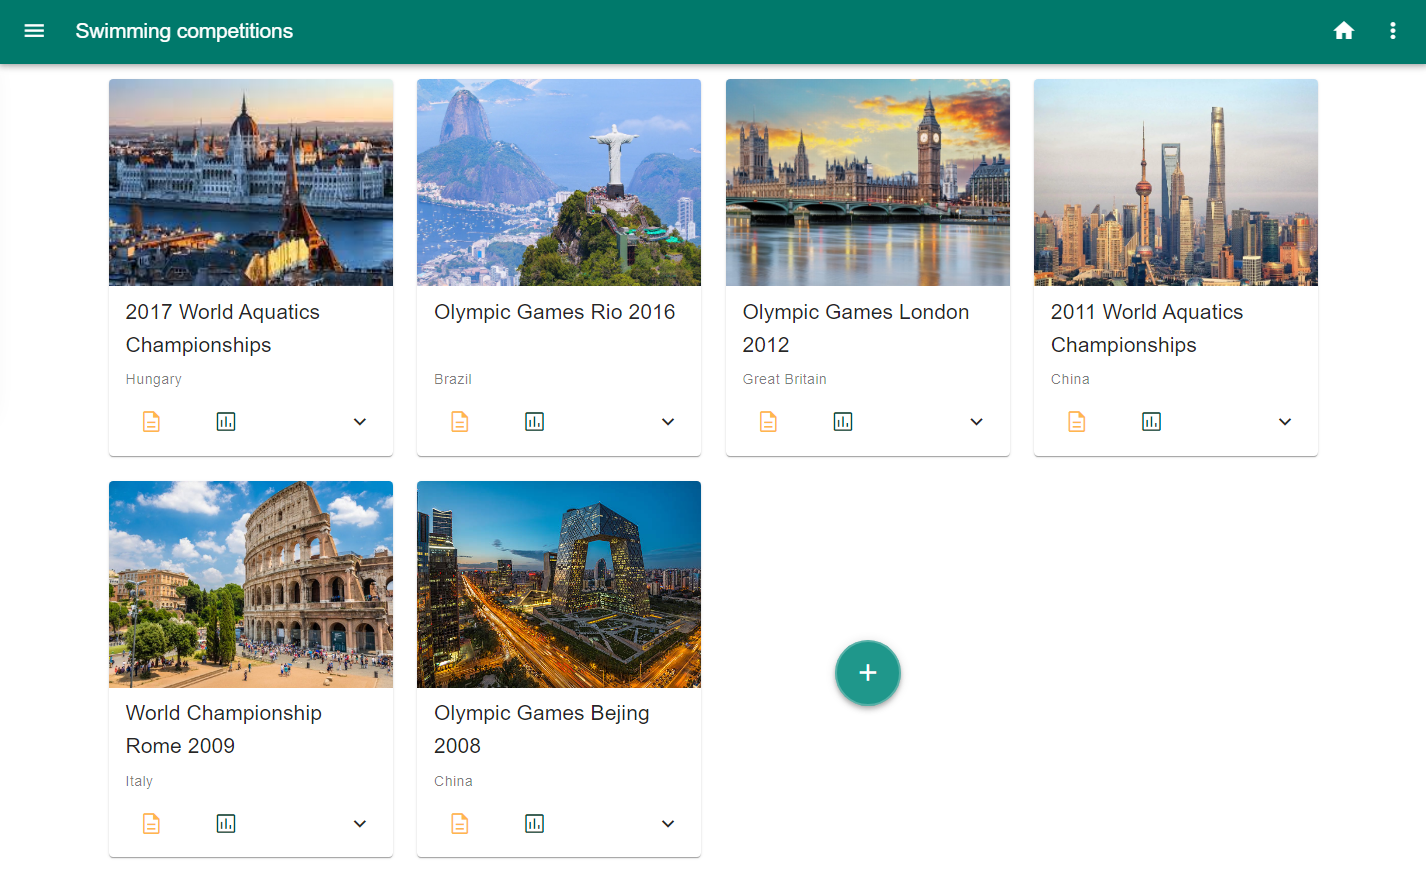
\includegraphics[width=15cm, height=10cm, keepaspectratio]{competition-add.png}
    \centering
    \caption{Kartica s prikazom svih natjecanja}
    \label{fig:competition-add}
\end{figure}

\begin{figure}[!h]
    \centering
    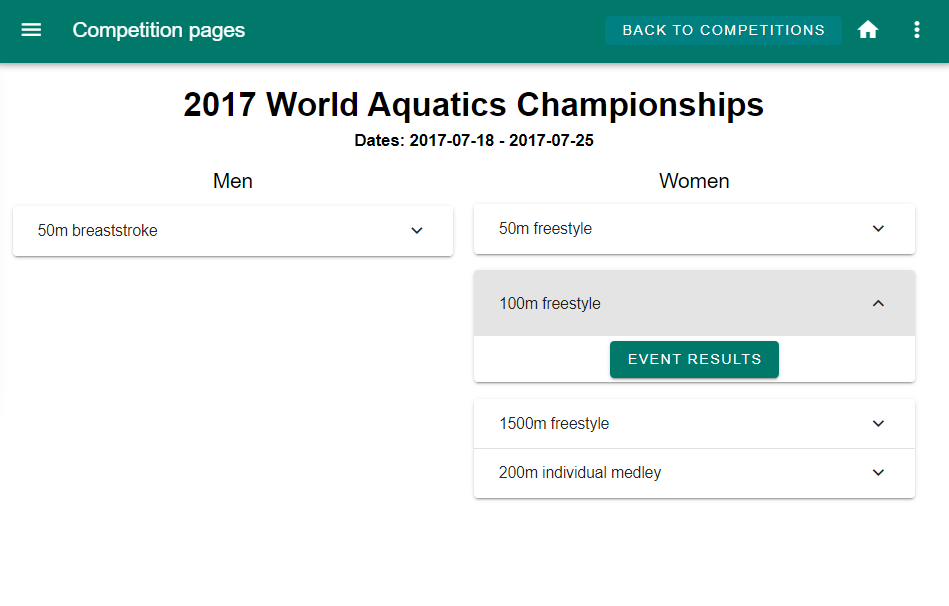
\includegraphics[width=10cm, height=10cm, keepaspectratio]{competition-details.png}
    \centering
    \caption{Kartica s prikazom detalja o odabranom natjecanju}
    \label{fig:competition-details}
\end{figure}

Na kraju liste prikaza natjecanja nalazi se gumb za dodavanje novog natjecanja. Korisniku se klikom na gumb prikazuje forma (slika \ref{fig:competition-form})
za dodavanje novog natjecanja.

\begin{figure}[!h]
    \centering
    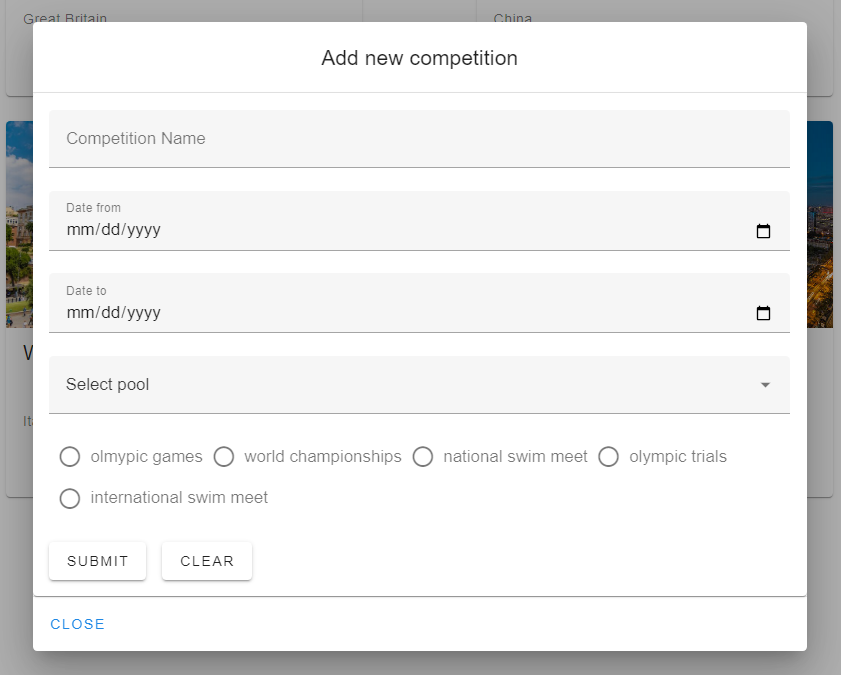
\includegraphics[width=10cm, height=8cm, keepaspectratio]{competition-form.png}
    \centering
    \caption{Forma za dodavanje novog natjecanja}
    \label{fig:competition-form}
\end{figure}

\subsection{Kvalificirani plivači}
Odabirom kartice kvalificirani plivači prikazuje se popis kvalificiranih plivača i discipline u kojima su se kvalificirali
Na dnu stranice pritiskom na gumb (slika \ref{fig:qualified-athletes}). Limiti prikazat će se limiti po disciplinama.

\begin{figure}[!h]
    \centering
    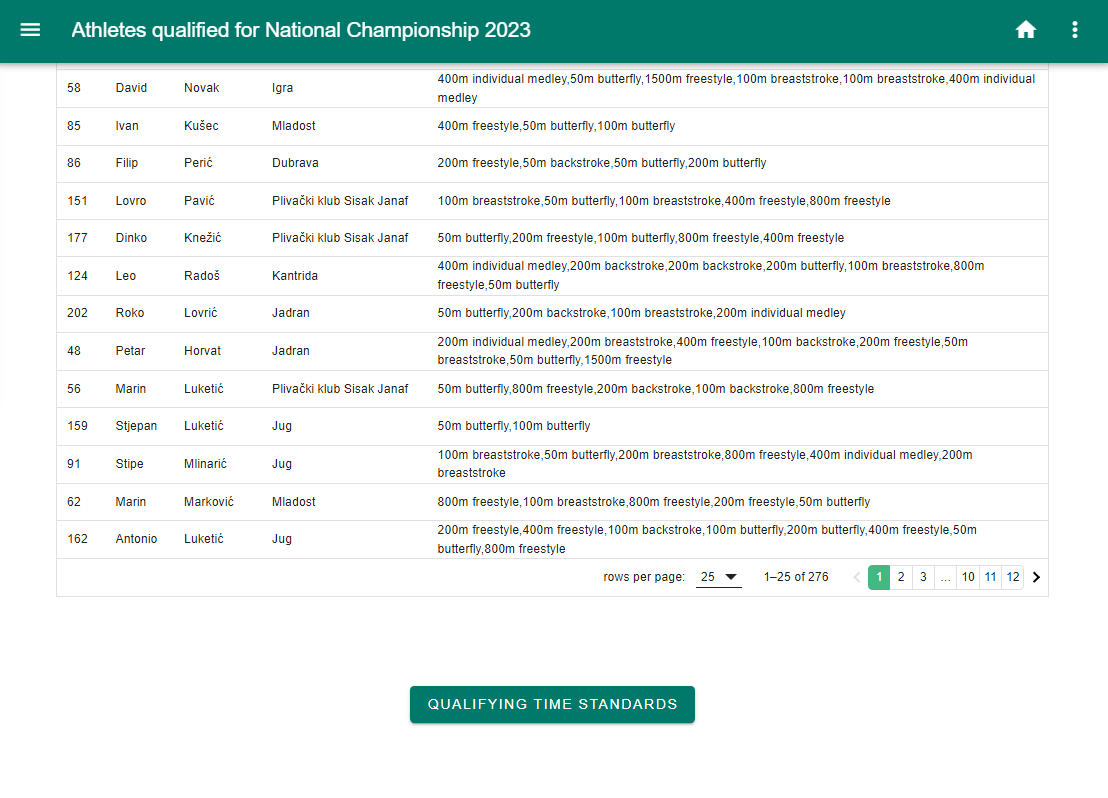
\includegraphics[width=14cm, height=10cm, keepaspectratio]{qualified-athletes.png}
    \centering
    \caption{Kartica s prikazom kvalificiranih plivača i limita}
    \label{fig:qualified-athletes}
\end{figure}

\subsection{Plivači}
Odabirom kartice plivači prikazuje se polje za unos teksta u koje korisnik treba unijeti ime traženog plivača (slika \ref{fig:swimmers}).
Pritiskom na gumb Traži otvara se starnica sa detaljima o traženom plivaču i njegovim najboljim rezultatima (slika \ref{fig:swimmers-page}).

\begin{figure}[!h]
    \centering
    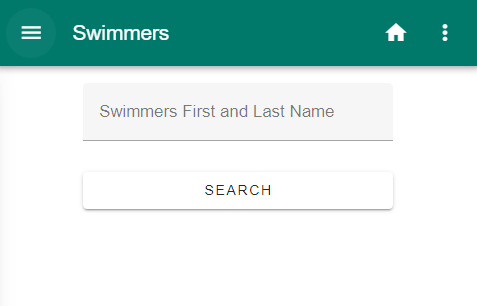
\includegraphics[width=8cm, height=8cm, keepaspectratio]{swimmers.png}
    \centering
    \caption{Kartica za pretraživanje plivača}
    \label{fig:swimmers}
\end{figure}

\begin{figure}[!h]
    \centering
    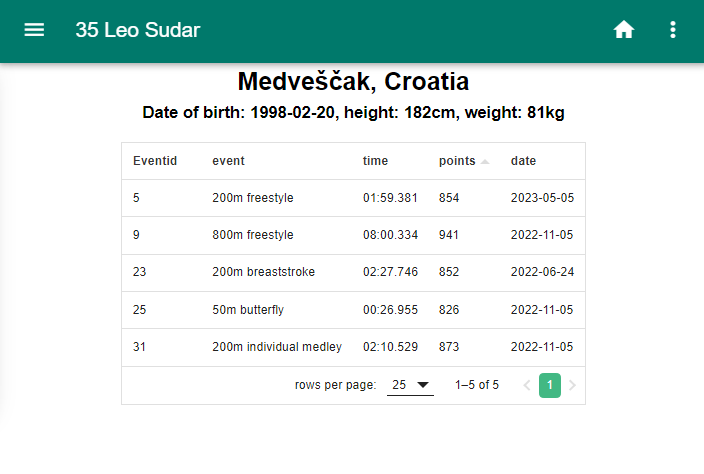
\includegraphics[width=12cm, height=12cm, keepaspectratio]{swimmers-page.png}
    \centering
    \caption{Kartica s prikazom detalja o plivaču}
    \label{fig:swimmers-page}
\end{figure}

\subsection{Bazeni}
Odabirom kartice bazeni prikazuje se popis registriranih bazena. Pritiskom na strelicu na kartici bazena prikazuju se detalji o pojedinom bazenu (slika \ref*{fig:pool}).

\begin{figure}[!h]
    \centering
    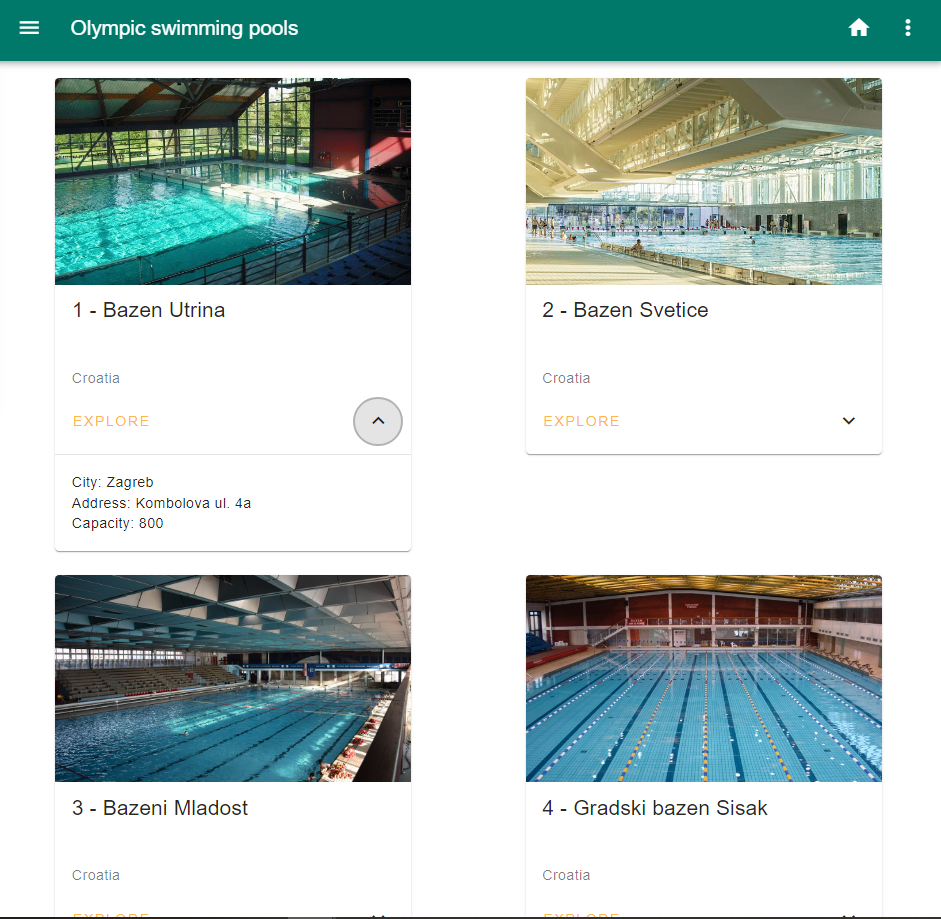
\includegraphics[width=12cm, height=12cm, keepaspectratio]{pool.png}
    \centering
    \caption{Kartica s prikazom svih bazena}
    \label{fig:pool}
\end{figure}

\subsection{Svjetski rekordi}
Odabirom kartice Svjetski rekordi prikazuje se popis svjetskih rekorda u pojedinoj disciplini (slika \ref*{fig:world-records}).

\begin{figure}[!h]
    \centering
    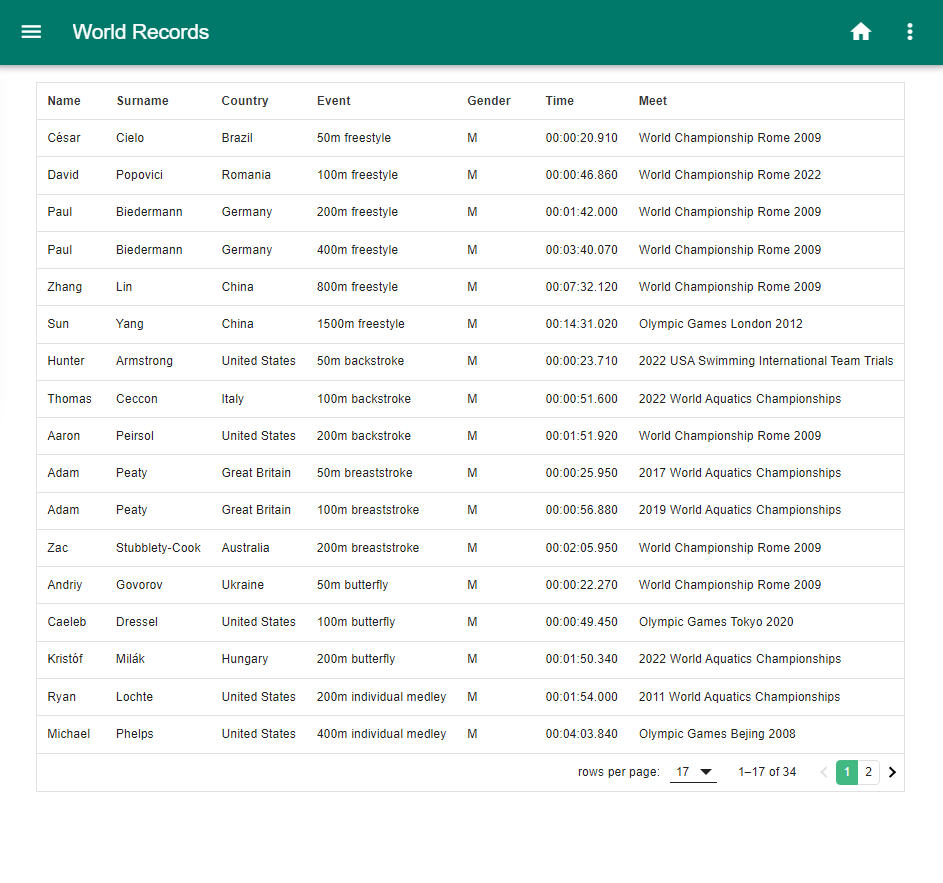
\includegraphics[width=15cm, height=10cm, keepaspectratio]{world-records.png}
    \centering
    \caption{Kartica s prikazom svjetskih rekorda}
    \label{fig:world-records}
\end{figure}

\chapter{Zaključak}
Web aplikacija za praćenje plivačkih rezultata i pregledavnje podataka o plivačkim natjecanjima uspješno je ostvarena
uporabom navedenih alata i tehnologija. Ova aplikacija je intuitivna za korištenjem sadašnjim, bivšim ili budućim
plivačima, ali i ljubiteljima plivanja. Ostvareno je jednostavno korisničko sučelje za prikaz navedenih podataka.

\vspace{\baselineskip}

Razvoj sustava podijelio sam u dvije faza: modeliranje i implementacija baze podataka, te pisanje koda za
razvoj web aplikacije. 

\vspace{\baselineskip}

Aplikacije bi se mogla unaprijediti dodavanjem različitih korisnika i trenera koji bi mogli mijenjati i unositi podatke.
Također bi se mogla dodati opcija usporedbe dvaju plivača na temelju njihovih rezultata ili graf prikaza napreetka
plivača kroz godine. Takve opcije bi omogćile plivačima da prate svoj napredak i imaju uvid u sve svoje rezultate.

\vspace{\baselineskip}

Rad na projektu mi se svidio jer je ovo prva veća aplikacija koju sam samostalno izradio. Izrada se pokazala kao vrlo
poučno iskustvo jer sam usavršio vec poznate tehnologije i naučio nove koje ću moći primjenjivati u budućimm projektima.
Smatram da je znanje stečeno u izradi praktičnog proizvoda korisnije od teorijskog znanja te se osjećam samopuzdanije u svoje
programerske sposobnosti. 

\citation{oetiket2007lshort}

\bibliography{literatura}
\bibliographystyle{fer}

\begin{sazetak}
Sažetak na hrvatskom jeziku.

\kljucnerijeci{Ključne riječi, odvojene zarezima.}
\end{sazetak}

% TODO: Navedite naslov na engleskom jeziku.
\engtitle{Title}
\begin{abstract}
Abstract.

\keywords{Keywords.}
\end{abstract}

\end{document}
